
%% bare_conf.tex
%% V1.3
%% 2007/01/11
%% by Michael Shell
%% See:
%% http://www.michaelshell.org/
%% for current contact information.
%%
%% This is a skeleton file demonstrating the use of IEEEtran.cls
%% (requires IEEEtran.cls version 1.7 or later) with an IEEE conference paper.
%%
%% Support sites:
%% http://www.michaelshell.org/tex/ieeetran/
%% http://www.ctan.org/tex-archive/macros/latex/contrib/IEEEtran/
%% and
%% http://www.ieee.org/

%%*************************************************************************
%% Legal Notice:
%% This code is offered as-is without any warranty either expressed or
%% implied; without even the implied warranty of MERCHANTABILITY or
%% FITNESS FOR A PARTICULAR PURPOSE!
%% User assumes all risk.
%% In no event shall IEEE or any contributor to this code be liable for
%% any damages or losses, including, but not limited to, incidental,
%% consequential, or any other damages, resulting from the use or misuse
%% of any information contained here.
%%
%% All comments are the opinions of their respective authors and are not
%% necessarily endorsed by the IEEE.
%%
%% This work is distributed under the LaTeX Project Public License (LPPL)
%% ( http://www.latex-project.org/ ) version 1.3, and may be freely used,
%% distributed and modified. A copy of the LPPL, version 1.3, is included
%% in the base LaTeX documentation of all distributions of LaTeX released
%% 2003/12/01 or later.
%% Retain all contribution notices and credits.
%% ** Modified files should be clearly indicated as such, including  **
%% ** renaming them and changing author support contact information. **
%%
%% File list of work: IEEEtran.cls, IEEEtran_HOWTO.pdf, bare_adv.tex,
%%                    bare_conf.tex, bare_jrnl.tex, bare_jrnl_compsoc.tex
%%*************************************************************************

% *** Authors should verify (and, if needed, correct) their LaTeX system  ***
% *** with the testflow diagnostic prior to trusting their LaTeX platform ***
% *** with production work. IEEE's font choices can trigger bugs that do  ***
% *** not appear when using other class files.                            ***
% The testflow support page is at:
% http://www.michaelshell.org/tex/testflow/



% Note that the a4paper option is mainly intended so that authors in
% countries using A4 can easily print to A4 and see how their papers will
% look in print - the typesetting of the document will not typically be
% affected with changes in paper size (but the bottom and side margins will).
% Use the testflow package mentioned above to verify correct handling of
% both paper sizes by the user's LaTeX system.
%
% Also note that the "draftcls" or "draftclsnofoot", not "draft", option
% should be used if it is desired that the figures are to be displayed in
% draft mode.
%


\documentclass[conference]{IEEEtran}

% Add the compsoc option for Computer Society conferences.
%
% If IEEEtran.cls has not been installed into the LaTeX system files,
% manually specify the path to it like:
% \documentclass[conference]{../sty/IEEEtran}



% Some very useful LaTeX packages include:
% (uncomment the ones you want to load)


% *** MISC UTILITY PACKAGES ***
%
%\usepackage{ifpdf}
% Heiko Oberdiek's ifpdf.sty is very useful if you need conditional
% compilation based on whether the output is pdf or dvi.
% usage:
% \ifpdf
%   % pdf code
% \else
%   % dvi code
% \fi
% The latest version of ifpdf.sty can be obtained from:
% http://www.ctan.org/tex-archive/macros/latex/contrib/oberdiek/
% Also, note that IEEEtran.cls V1.7 and later provides a builtin
% \ifCLASSINFOpdf conditional that works the same way.
% When switching from latex to pdflatex and vice-versa, the compiler may
% have to be run twice to clear warning/error messages.



% *** CITATION PACKAGES ***
%
%\usepackage{cite}
% cite.sty was written by Donald Arseneau
% V1.6 and later of IEEEtran pre-defines the format of the cite.sty package
% \cite{} output to follow that of IEEE. Loading the cite package will
% result in citation numbers being automatically sorted and properly
% "compressed/ranged". e.g., [1], [9], [2], [7], [5], [6] without using
% cite.sty will become [1], [2], [5]--[7], [9] using cite.sty. cite.sty's
% \cite will automatically add leading space, if needed. Use cite.sty's
% noadjust option (cite.sty V3.8 and later) if you want to turn this off.
% cite.sty is already installed on most LaTeX systems. Be sure and use
% version 4.0 (2003-05-27) and later if using hyperref.sty. cite.sty does
% not currently provide for hyperlinked citations.
% The latest version can be obtained at:
% http://www.ctan.org/tex-archive/macros/latex/contrib/cite/
% The documentation is contained in the cite.sty file itself.




\usepackage{listings}

% *** GRAPHICS RELATED PACKAGES ***
%
\ifCLASSINFOpdf
\usepackage[pdftex]{graphicx}
\usepackage[pdftex]{color}
\usepackage{subcaption}
\usepackage{url}
  % declare the path(s) where your graphic files are
\graphicspath{{./images}}
  % and their extensions so you won't have to specify these with
  % every instance of \includegraphics
  % \DeclareGraphicsExtensions{.pdf,.jpeg,.png}
\else
  % or other class option (dvipsone, dvipdf, if not using dvips). graphicx
  % will default to the driver specified in the system graphics.cfg if no
  % driver is specified.
  % \usepackage[dvips]{graphicx}
  % declare the path(s) where your graphic files are
  % \graphicspath{{../eps/}}
  % and their extensions so you won't have to specify these with
  % every instance of \includegraphics
  % \DeclareGraphicsExtensions{.eps}
\fi
% graphicx was written by David Carlisle and Sebastian Rahtz. It is
% required if you want graphics, photos, etc. graphicx.sty is already
% installed on most LaTeX systems. The latest version and documentation can
% be obtained at:
% http://www.ctan.org/tex-archive/macros/latex/required/graphics/
% Another good source of documentation is "Using Imported Graphics in
% LaTeX2e" by Keith Reckdahl which can be found as epslatex.ps or
% epslatex.pdf at: http://www.ctan.org/tex-archive/info/
%
% latex, and pdflatex in dvi mode, support graphics in encapsulated
% postscript (.eps) format. pdflatex in pdf mode supports graphics
% in .pdf, .jpeg, .png and .mps (metapost) formats. Users should ensure
% that all non-photo figures use a vector format (.eps, .pdf, .mps) and
% not a bitmapped formats (.jpeg, .png). IEEE frowns on bitmapped formats
% which can result in "jaggedy"/blurry rendering of lines and letters as
% well as large increases in file sizes.
%
% You can find documentation about the pdfTeX application at:
% http://www.tug.org/applications/pdftex





% *** MATH PACKAGES ***
%
%\usepackage[cmex10]{amsmath}
% A popular package from the American Mathematical Society that provides
% many useful and powerful commands for dealing with mathematics. If using
% it, be sure to load this package with the cmex10 option to ensure that
% only type 1 fonts will utilized at all point sizes. Without this option,
% it is possible that some math symbols, particularly those within
% footnotes, will be rendered in bitmap form which will result in a
% document that can not be IEEE Xplore compliant!
%
% Also, note that the amsmath package sets \interdisplaylinepenalty to 10000
% thus preventing page breaks from occurring within multiline equations. Use:
%\interdisplaylinepenalty=2500
% after loading amsmath to restore such page breaks as IEEEtran.cls normally
% does. amsmath.sty is already installed on most LaTeX systems. The latest
% version and documentation can be obtained at:
% http://www.ctan.org/tex-archive/macros/latex/required/amslatex/math/





% *** SPECIALIZED LIST PACKAGES ***
%
%\usepackage{algorithmic}
% algorithmic.sty was written by Peter Williams and Rogerio Brito.
% This package provides an algorithmic environment fo describing algorithms.
% You can use the algorithmic environment in-text or within a figure
% environment to provide for a floating algorithm. Do NOT use the algorithm
% floating environment provided by algorithm.sty (by the same authors) or
% algorithm2e.sty (by Christophe Fiorio) as IEEE does not use dedicated
% algorithm float types and packages that provide these will not provide
% correct IEEE style captions. The latest version and documentation of
% algorithmic.sty can be obtained at:
% http://www.ctan.org/tex-archive/macros/latex/contrib/algorithms/
% There is also a support site at:
% http://algorithms.berlios.de/index.html
% Also of interest may be the (relatively newer and more customizable)
% algorithmicx.sty package by Szasz Janos:
% http://www.ctan.org/tex-archive/macros/latex/contrib/algorithmicx/




% *** ALIGNMENT PACKAGES ***
%
%\usepackage{array}
% Frank Mittelbach's and David Carlisle's array.sty patches and improves
% the standard LaTeX2e array and tabular environments to provide better
% appearance and additional user controls. As the default LaTeX2e table
% generation code is lacking to the point of almost being broken with
% respect to the quality of the end results, all users are strongly
% advised to use an enhanced (at the very least that provided by array.sty)
% set of table tools. array.sty is already installed on most systems. The
% latest version and documentation can be obtained at:
% http://www.ctan.org/tex-archive/macros/latex/required/tools/


%\usepackage{mdwmath}
%\usepackage{mdwtab}
% Also highly recommended is Mark Wooding's extremely powerful MDW tools,
% especially mdwmath.sty and mdwtab.sty which are used to format equations
% and tables, respectively. The MDWtools set is already installed on most
% LaTeX systems. The lastest version and documentation is available at:
% http://www.ctan.org/tex-archive/macros/latex/contrib/mdwtools/


% IEEEtran contains the IEEEeqnarray family of commands that can be used to
% generate multiline equations as well as matrices, tables, etc., of high
% quality.


%\usepackage{eqparbox}
% Also of notable interest is Scott Pakin's eqparbox package for creating
% (automatically sized) equal width boxes - aka "natural width parboxes".
% Available at:
% http://www.ctan.org/tex-archive/macros/latex/contrib/eqparbox/





% *** SUBFIGURE PACKAGES ***
%\usepackage[tight,footnotesize]{subfigure}
% subfigure.sty was written by Steven Douglas Cochran. This package makes it
% easy to put subfigures in your figures. e.g., "Figure 1a and 1b". For IEEE
% work, it is a good idea to load it with the tight package option to reduce
% the amount of white space around the subfigures. subfigure.sty is already
% installed on most LaTeX systems. The latest version and documentation can
% be obtained at:
% http://www.ctan.org/tex-archive/obsolete/macros/latex/contrib/subfigure/
% subfigure.sty has been superceeded by subfig.sty.



%\usepackage[caption=false]{caption}
%\usepackage[font=footnotesize]{subfig}
% subfig.sty, also written by Steven Douglas Cochran, is the modern
% replacement for subfigure.sty. However, subfig.sty requires and
% automatically loads Axel Sommerfeldt's caption.sty which will override
% IEEEtran.cls handling of captions and this will result in nonIEEE style
% figure/table captions. To prevent this problem, be sure and preload
% caption.sty with its "caption=false" package option. This is will preserve
% IEEEtran.cls handing of captions. Version 1.3 (2005/06/28) and later
% (recommended due to many improvements over 1.2) of subfig.sty supports
% the caption=false option directly:
%\usepackage[caption=false,font=footnotesize]{subfig}
%
% The latest version and documentation can be obtained at:
% http://www.ctan.org/tex-archive/macros/latex/contrib/subfig/
% The latest version and documentation of caption.sty can be obtained at:
% http://www.ctan.org/tex-archive/macros/latex/contrib/caption/




% *** FLOAT PACKAGES ***
%
%\usepackage{fixltx2e}
% fixltx2e, the successor to the earlier fix2col.sty, was written by
% Frank Mittelbach and David Carlisle. This package corrects a few problems
% in the LaTeX2e kernel, the most notable of which is that in current
% LaTeX2e releases, the ordering of single and double column floats is not
% guaranteed to be preserved. Thus, an unpatched LaTeX2e can allow a
% single column figure to be placed prior to an earlier double column
% figure. The latest version and documentation can be found at:
% http://www.ctan.org/tex-archive/macros/latex/base/



%\usepackage{stfloats}
% stfloats.sty was written by Sigitas Tolusis. This package gives LaTeX2e
% the ability to do double column floats at the bottom of the page as well
% as the top. (e.g., "\begin{figure*}[!b]" is not normally possible in
% LaTeX2e). It also provides a command:
%\fnbelowfloat
% to enable the placement of footnotes below bottom floats (the standard
% LaTeX2e kernel puts them above bottom floats). This is an invasive package
% which rewrites many portions of the LaTeX2e float routines. It may not work
% with other packages that modify the LaTeX2e float routines. The latest
% version and documentation can be obtained at:
% http://www.ctan.org/tex-archive/macros/latex/contrib/sttools/
% Documentation is contained in the stfloats.sty comments as well as in the
% presfull.pdf file. Do not use the stfloats baselinefloat ability as IEEE
% does not allow \baselineskip to stretch. Authors submitting work to the
% IEEE should note that IEEE rarely uses double column equations and
% that authors should try to avoid such use. Do not be tempted to use the
% cuted.sty or midfloat.sty packages (also by Sigitas Tolusis) as IEEE does
% not format its papers in such ways.





% *** PDF, URL AND HYPERLINK PACKAGES ***
%
\usepackage{url}
% url.sty was written by Donald Arseneau. It provides better support for
% handling and breaking URLs. url.sty is already installed on most LaTeX
% systems. The latest version can be obtained at:
% http://www.ctan.org/tex-archive/macros/latex/contrib/misc/
% Read the url.sty source comments for usage information. Basically,
% \url{my_url_here}.





% *** Do not adjust lengths that control margins, column widths, etc. ***
% *** Do not use packages that alter fonts (such as pslatex).         ***
% There should be no need to do such things with IEEEtran.cls V1.6 and later.
% (Unless specifically asked to do so by the journal or conference you plan
% to submit to, of course. )


% correct bad hyphenation here
\hyphenation{}


\begin{document}
%
% paper title
% can use linebreaks \\ within to get better formatting as desired
\title{SpyREST: Automated Example Based Documentation for RESTful Web APIs}


% author names and affiliations
% use a multiple column layout for up to three different
% affiliations
\author{\IEEEauthorblockN{S M Sohan}
\IEEEauthorblockA{Department of Computer Science\\
University of Calgary\\
Calgary, Alberta T2N 1N4\\
Email: http://smsohan.com/home}
}
% \and
% \IEEEauthorblockN{Homer Simpson}
% \IEEEauthorblockA{Twentieth Century Fox\\
% Springfield, USA\\
% Email: homer@thesimpsons.com}
% \and
% \IEEEauthorblockN{James Kirk\\ and Montgomery Scott}
% \IEEEauthorblockA{Starfleet Academy\\
% San Francisco, California 96678-2391\\
% Telephone: (800) 555--1212\\
% Fax: (888) 555--1212}}

% conference papers do not typically use \thanks and this command
% is locked out in conference mode. If really needed, such as for
% the acknowledgment of grants, issue a \IEEEoverridecommandlockouts
% after \documentclass

% for over three affiliations, or if they all won't fit within the width
% of the page, use this alternative format:
%
%\author{\IEEEauthorblockN{Michael Shell\IEEEauthorrefmark{1},
%Homer Simpson\IEEEauthorrefmark{2},
%James Kirk\IEEEauthorrefmark{3},
%Montgomery Scott\IEEEauthorrefmark{3} and
%Eldon Tyrell\IEEEauthorrefmark{4}}
%\IEEEauthorblockA{\IEEEauthorrefmark{1}School of Electrical and Computer Engineering\\
%Georgia Institute of Technology,
%Atlanta, Georgia 30332--0250\\ Email: see http://www.michaelshell.org/contact.html}
%\IEEEauthorblockA{\IEEEauthorrefmark{2}Twentieth Century Fox, Springfield, USA\\
%Email: homer@thesimpsons.com}
%\IEEEauthorblockA{\IEEEauthorrefmark{3}Starfleet Academy, San Francisco, California 96678-2391\\
%Telephone: (800) 555--1212, Fax: (888) 555--1212}
%\IEEEauthorblockA{\IEEEauthorrefmark{4}Tyrell Inc., 123 Replicant Street, Los Angeles, California 90210--4321}}




% use for special paper notices
%\IEEEspecialpapernotice{(Invited Paper)}




% make the title area
\maketitle


\begin{abstract}
Documentation of RESTful APIs are expensive to produce and maintain. It is expensive because there is a lack of reusable tools and automated solutions for RESTful API documentation. Most RESTful APIs are documented manually and the API developers are responsible for keeping an updated documentation as the API evolves making the process both costly and error-prone. In this paper we introduce SpyREST, a reusable tool that can automatically generate RESTful API documentation. SpyREST uses a proxy to intercept example API calls and intelligently produces API documentation for RESTful Web APIs by processing the request and response data. Using SpyREST, RESTful API developers can significantly reduce the cost of producing and maintaining API documentation by replacing a large part of the manual process of documentation with an automated one.
\end{abstract}

% IEEEtran.cls defaults to using nonbold math in the Abstract.
% This preserves the distinction between vectors and scalars. However,
% if the conference you are submitting to favors bold math in the abstract,
% then you can use LaTeX's standard command \boldmath at the very start
% of the abstract to achieve this. Many IEEE journals/conferences frown on
% math in the abstract anyway.

% no keywords




% For peer review papers, you can put extra information on the cover
% page as needed:
% \ifCLASSOPTIONpeerreview
% \begin{center} \bfseries EDICS Category: 3-BBND \end{center}
% \fi
%
% For peerreview papers, this IEEEtran command inserts a page break and
% creates the second title. It will be ignored for other modes.
\IEEEpeerreviewmaketitle

\begin{IEEEkeywords}
RESTful API, Web API, Documentation, Automation, Example based documentation
\end{IEEEkeywords}


\section{Introduction}
RESTful APIs are used as a primary interconnection mechanism among modern day Web based systems. For example, the website of a restaurant can use the RESTful API from Twitter to show the latest tweets mentioning the restaurant so that prospective customers can read the experience shared by others. To allow others to use their APIs, Twitter and other RESTful API developers publish documentation describing different features of their RESTful API. The documentation of such RESTful APIs are commonly produced and maintained using a manual process.

API documentation for library APIs, such as Java Standard Edition, commonly leverage reusable tools such as JavaDoc. The documentation produced by such tools include description of objects and methods, with custom texts primarily sourced via comments. On the other hand, RESTful APIs documentation includes additional information such as HTTP headers, request parameters, request and response data in serialized formats such as JSON, XML that cannot be easily derived from looking at the objects and methods in the source code. Using comments for these additional information also requires significant manual effort because there is a lack of reusable tools to automate the documentation process. This makes the task of RESTful API documentation a costly and error-prone one. In addition to producing the API documentation, API developers also need to publish and often maintain the documentation for multiple versions as the RESTful API evolves. This requires further manual effort because it becomes a continuous process.

To produce RESTful API documentation with information about HTTP headers, URL parameters, request and response data, the manual process is driven by example API calls. Example calls are made and recorded against an API endpoint to gather information for documentation. This process can be described as a six-step process as follows: 1) craft an example call to an API endpoint with required headers, URL parameters and request body, 2) make the call, 3) capture the response headers and data, 4) strip any unwanted data from the captured information, 5) add custom descriptions to the captured data and 6) publish the API documentation. This six-step process is essentially repeated for all API endpoints that are documented.

With SpyREST, we have implemented an innovative solution to largely automate the aforementioned manual process of RESTful API documentation so that all but steps 1 and 5 are automated. Steps 1 and 5 are left to a manual process to allow for a pragmatic solution that leverages computers to automate the repeated part of the process while leaving the rest to humans. Our solution relies on a lightweight HTTP proxy server to intercept example API calls so that all the information about HTTP headers, URL parameters, request and response data can be automatically gathered. The collected data is then processed to present the documentation for RESTful resources under a hierarchy defined by API versions, resources and actions. Sensitive data such as authentication tokens and passwords are automatically filtered and are not captured. Because SpyREST uses a HTTP proxy server, it can generate documentation for all RESTful APIs irrespective of the technology used to implement the API. The resultant is an automated yet customizable, version-aware, collaboration enabled and reusable API documentation software as a service platform that can be used to generate and maintain documentation for any RESTful API.

The implication of SpyREST is two-fold. It helps lower the cost of producing and maintaining RESTful API documentation through automation and provides a shared platform for publishing the documentation of different RESTful APIs.

The remainder of this paper is organized as follows: in the next section we discuss the related work on API documentation. The implementation details of SpyREST is provided next. Then, we present a case study to demonstrate SpyREST in action. Then, we discuss the implications and limitations of our work in the discussion section. We present our core contributions and future work in the conclusion.


\section{Related Work} % (fold)
\label{sec:related_work}
Several papers have been published on areas related to RESTful API documentation that are discussed under the following two categories: general API documentation and RESTful API documentation.

\subsection{General API Documentation} % (fold)
\label{ssub:api_learnability}
Several papers have studied the documentation of APIs to understand and recommend best practices that are also applicable to RESTful API documentation. Robillard et al. discussed the obstacles that make APIs hard to learn by surveying API developers and users \cite{Robillard_what_makes} \cite{Robillard_a_field_study}. They found that  developers faced severe obstacles learning new APIs due to inappropriate documentation and other learning resources. Robillard's recommendations for good API documentations include the following: include good examples, be complete, support many complex usage scenarios, be conveniently organized, and include relevant design elements. Kuhn et al. discussed the importance of good examples in API documentation as a key recommendation based on a survey of software developers using APIs \cite{Kuhn_on_designing}. In addition to examples, they identified trustworthiness, confidentiality, and limiting information overload as other key recommendations for API documentation. When API documentation is published for external use, Kuhn identified the need for the documentation tools to be able to protect proprietary and confidential information. Hoffman et al. recommended making the API example scenarios to be executable test cases so that a user can execute an API and understand the related business rules \cite{Hoffman_api_documentation}. We recognize all these recommendations to be equally important for RESTful APIs. SpyREST automatically generates RESTful API documents from example API calls, with information about the publisher and allows the users to execute the examples following the aforementioned recommendations.

Nasehi et al. performed a case study based on StackOverflow discussions to find out what makes good code examples \cite{Nasehi_what_makes}. They recommended API developers to include a comprehensive set of code examples in the API documentation and the use of wiki-like collaborative tools with online API documentation so that users can ask questions and get answers on officially published API documentation. Parnin et al. found that social media holds a key place in software documentation as  it provides additional knowledge about APIs and gives readers a chance to engage with authors of the APIs \cite{Parnin_measuring}. They found active collaboration about API related questions resulting into 81\% of posts receiving at least one comment with a median of 8 comments per question. Chen et al. recommended integrating crowdsourced frequently asked questions (FAQs) into API documents so that users can easily find relevant discussions when questions arise as they are browsing API documentation \cite{Chen_who_asked}. They presented a tool that can embed FAQs into API documents based on a user's browsing behavior. Subramanian et al. presented an automated approach to link API documentation of different Java and JavaScript libraries with code examples that are shared on StackOverflow by the API users so that the collaborative crowd documentation of APIs can be linked with official documentations \cite{Subramanian_live}. To link API documentation with valuable crowdsourced content, the collaborative features of SpyREST allows users to discuss API related questions and answers on the same web pages where the auto generated RESTful API documentations are shown.

Stepalina discussed the advantages of SaaS based solutions for API documentation systems where a web platform can be used to publish many different API documentations \cite{Stepalina_saas}. They identified several benefits of such a reusable platform, such as, cost effective yet powerful, platform agnostic and high accessibility, improved document quality, content re-use, automated tools and organization of robust and scalable documentation process. SpyREST is a SaaS based tool that can be used to leverage these benefits as it allows the generation and publishing of RESTful API documentations for many different APIs under a single platform. They also identified security and reliability of such a shared platform as potentially open issues. To overcome these issues, SpyREST allows a self hosted alternative to SaaS model where API developers can get full isolation for their RESTful API documentation.

Several tools exist that help automatic generation of API documentation for local APIs such as JavaDoc \footnote{http://www.oracle.com/technetwork/java/javase/documentation/index-jsp-135444.html}, RDoc \footnote{http://rdoc.sourceforge.net/} etc. that convert formatted comments from source code into corresponding HTML documentation for the classes and methods. Jadeite is a tool that adds placeholder API objects for library APIs to improve the search and discovery of desired API objects \cite{Jadeite}. While these tools have been proven to work for local library APIs, they have a limited applicability for documenting RESTful APIs because HTTP specific information such as request and response headers, url, request and response payloads are not natively supported by these tools. Hence, there exists a gap for tool support to automatically generate RESTful API documentation. SpyREST fills this gap as it automatically generates RESTful API documentation by recording and synthesizing example API calls.

\subsection{RESTful API Documentation} % (fold)
\label{sub:restful_api_documentation}

To address the need for a standard format to describe RESTful APIs several related works proposed candidate specifications. For example, Danielsen et al. presented at vocabulary for documenting RESTful Web APIs called Web Interface Language (WIfL) \cite{Danielsen_validation}. The vocabulary comprises of these following objects: Resource, Request, Response, Representation and Parameters that can describe the structure and example usage of RESTful Web APIs. Generation of WIfL specific objects for RESTful APIs requires manual effort or bespoke implementation since a reusable automated approach is not presented. With SpyREST, we focus on automation so that reusable tools can be used to produce RESTful API documentation.

Verborgh et at. presented RESTdesc, a Resource oriented and Hyper-link based specification for describing RESTful APIs \cite{Verborgh_functional}. RESTdesc relies on pre and postconditions to describe the outcome of an API call so that a general purpose API client can parse RESTdesc formatted documentation to invoke API calls to specific RESTful APIs. Mangler et al. presented RDDL, a XML based specification for describing RESTful APIs \cite{Mangler_rddl}. RDDL descriptions are composed of resources, operations, parameters and headers. Similar to WIfl, manual effort is needed to generate RESTdesc and RDDL formatted documentations.

Kopecky´ et al. presented hRESTS, a machine readable micro-format to describe RESTful APIs that uses an alternate representation compared to WIfL \cite{Kopecky_hrests}. hRESTS specification comprises of Service, Operation, Address, Method, Input, Output and Label objects to describe RESTful APIs. Automated XML transformation is used to convert a formatted HTML documentation of a RESTful API into hRESTS so that the machine readable format can be used by RESTful API clients for automated invocation. SpyREST aims to minimize the cost of a manual or custom process to generate and maintain formatted HTML documentation by leveraging an automated approach.

Maleshkova et al. presented OmniVoke, a RESTful API based invocation engine that provides an abstraction layer for RESTful API calls to multiple APIs that follow different conventions \cite{Maleshkova_omnivoke}. A general purpose RESTful API client can be used against OmniVoke since the different conventions are wrapped under a uniform RESTful API. Manual configuration is required for each existing API to wrap under OmniVoke.

Myers et al. performed a user study based on the documentation of Web APIs used in large scale enterprises to understand the desirable contents for Web API documentation \cite{Myers_study}. They recommended providing a consistent look-and-feel with explanation for the starting points and an overall map comprising of both text and diagrams, providing a browsing experience with breadcrumb trail following a hierarchy, an effective search interface, providing example code and a way to exercise the examples online without writing code. SpyREST aims to achieve requirements for RESTful API documentation using an automated yet customizable approach that can be reused across different RESTful APIs.

In addition to the research community, there are several RESTful API specification formats that are observed in the industry. Swagger is a JSON based specification that allows users to describe RESTful APIs in terms of paths, parameters, request and response headers and bodies \footnote{https://github.com/swagger-api/swagger-spec/blob/master/versions/2.0.md}. RAML is a RESTful API documentation format that uses YAML files to describe RESTful API documentation using a similar hierarchy as Swagger \footnote{http://raml.org/spec.html}. Blueprint is another RESTful API specification format that uses Markdown files with additional tags to describe RESTful API objects \footnote{https://github.com/apiaryio/api-blueprint}. In addition to producing RESTful API documentation, there are tools and software as a service (SaaS) providers that can be used to publish the documentation and auto generate API client code for RESTful APIs that are described using one of these formats. To use these tools to generate HTML based RESTful API documentation, API developers need to manually construct the intermediate documentation format that is required by these platforms since there is no automated tool to produce this. In contrast, SpyREST generates RESTful API documentation by synthesizing data collected from example API calls without relying on any intermediate representation.
% subsubsection restful_api_specification (end)


\section{SpyREST} % (fold)
\label{sec:spyrest}

\subsection{SpyREST Requirements} % (fold)
\label{sub:spyrest_requirements}

The following list of requirements for SpyREST is derived from analyzing the aforementioned related work and current API documentation practices as observed in the industry:


  \textbf{Automated RESTful API documentation}: RESTful APIs are either documented manually or using custom tools to partially automate the process. Both processes can be expensive to maintain since API documentation is a continuous process to support the evolution of APIs. The primary requirement for SpyREST is to find a pragmatic approach to automatically generate RESTful API documentation.


  \textbf{Example based}: As discussed in the related work section, several authors have emphasized on including example scenarios with API documentation to help users understand how to use an API \cite{Robillard_what_makes} \cite{Kuhn_on_designing} \cite{Hoffman_api_documentation} \cite{Nasehi_what_makes}. SpyREST generated API documentation needs to include example scenarios.

  \textbf{Executable documentation}: In addition to including examples, SpyREST also needs to allow users to execute the example scenarios so that they can try the API features without having to write code as recommended in related work \cite{Hoffman_api_documentation} \cite{Myers_study}.

  \textbf{Version awareness}: SpyREST needs to allow API developers to publish documentation for multiple versions of a Web API as it evolves. The following comment from a API user of Stripe shows the importance of a version-aware documentation tool \footnote{\url{https://groups.google.com/a/lists.stripe.com/forum/#!searchin/api-discuss/version/api-discuss/li4PyVcweiw/NT9SFTtF-vQJ}}
:
  \small
  \begin{quotation}
   ``Does the full API documentation only reflect the current version of the
    API?  Is there a way to access the API docs for outdated versions? ...That would be very helpful. When you are trying to upgrade from one version to another it's impossible to know the implementation differences. We are currently about 4 API versions behind and are stuck behind a version that causes a significant amount of work on our end to support. I'd like to be able to upgrade incrementally through each version.''
  \end{quotation}
  \normalsize

  \textbf{Customizable}: Robillard identified the importance of customized overview information about how to use an API to reduce API learning obstacles \cite{Robillard_what_makes}. Custom content is also required to explain business rules and overview information about APIs that may not be automatically derivable. SpyREST needs to allow users to add customized content to auto generated RESTful API documentation to enrich the quality of the documentation.

  \textbf{Reusable}: SpyREST needs to work as a reusable platform so that multiple REST API documentations can be generated and published on a single platform to get the benefits as outlined by Stepalina \cite{Stepalina_saas}.

  \textbf{Collaborative}: SpyREST needs to allow people to collaborate on the API documentation so that questions and answers about APIs can coexist with the API documentation to overcome the obstacles with fragmented knowledge sources as identified by Chen et al. \cite{Chen_who_asked}.


\subsection{SpyREST Components} % (fold)
SpyREST is composed of three main components as shown in Fig. \ref{fig:components}.

\begin{figure}[htb]
\centering
\def\svgwidth{\linewidth}
\input{components.pdf_tex}
\caption{SpyREST Component Diagram}
\label{fig:components}
\end{figure}

\textbf{The Spy:} SpyREST is driven by example calls to the RESTful APIs to generate the documentation for the APIs. The Spy component is a HTTP proxy server that needs to be used while running example API calls so that it can record HTTP request and response information in a database that are required to auto generate the API documentation. For example, when using Spy as a HTTP proxy to make the following HTTP request:

\scriptsize
\begin{description}
  \item[Method] GET
  \item[URL] https://api.github.com/repositories?since=100
  \item[Headers] accept: application/vnd.github.v3+json
\end{description}
\normalsize
that produces the following response:
\scriptsize
\begin{description}
  \item[Headers] status: 200 OK \\
content-type: application/json; charset=utf-8 \\
...
  \item[Body]
\begin{lstlisting}

[
  {
    "id": 1,
    "name": "grit",
    "full_name": "mojombo/grit",
    ...
  }
]\end{lstlisting}
\end{description}
\normalsize
Spy automatically saves the raw request and response data with HTTP headers. Additionally, it synthesizes the data and saves the following meta data about this example API call:
\scalebox{0.7}{
\begin{tabular}{r l}
  version & v3 \\
  resource & repositories \\
  action & GET /repositories \\
  query & since: 100 \\
  strippedResponseBody & a subset of the response body \\
  description & blank \\
  digest & base64 hash value of the version, resource, url and description \\
  requiresAuth & false \\
  apiToken & blank, used when a SpyREST API token is provided \\
  userId & blank, used when a user is found for given apiToken \\
\end{tabular}
}

As shown in this example, the version ``v3'' is automatically detected by parsing the accept request header. The automatic version detection algorithm can extract version information from either the request URL or accept header for most commonly used formats. Next, the resource field is also auto detected as ``repositories'' by parsing the request URL. The action ``GET /repositories'' is automatically detected by combining the request HTTP method with request path. The strippedResponseBody field automatically saves a shorter version of the actual response where large arrays in the response body are recursively truncated to smaller arrays with two sample items to reduce noise from the generated documentation. These meta fields allow SpyREST to structure the example API calls for a given API host in a hierarchical model as follows: an API has many versions, each version has many resources, each resource has many actions, and each action has many examples.

Auto detection algorithms for version, resource and action fields may be overridden by providing SpyREST with additional headers when example API calls are executed. For example, a user can use the custom header ``x-spy-rest-resource: repos'' when making example API calls to override the automatic detection of resource from ``repositories'' to ``repos''. Using a similar approach, users can override the version, action, and description fields using the ``x-spy-rest-version'', ``x-spy-rest-action'' and ``x-spy-rest-description'' headers respectively.

The digest is automatically computed based on the version, resource, url and description fields. Using this digest, Spy allows the users to replay the the same example and update the recorded information without creating duplicate entries for each run of the same example API.

When saving request information, Spy automatically strips of values used in ``authorization'' request headers to avoid leaking secrets in the API documentation. If an authorization header is found, Spy also marks the example with ``requiresAuth: true'' so that in the generated API documentation it can be visually indicated.

SpyREST allows users to sign up and get an API key to be used for generating API documentation. The ``apiToken'' and ``userId'' fields are populated when a valid SpyREST API key is provided in the ``x-spy-rest-api-key'' request header. This provides credibility to the documentation generated by SpyREST since the official API developers can be identified by their SpyREST account.

To record data for an example call to an API that uses a SSL/TLS connection, the Spy needs to perform as an intentional man-in-the-middle style proxy since the data would be encrypted otherwise. We consider the security risks for this approach to be minimal when the example API calls are intended to be recorded for public viewing through the documentation. For APIs where this is not acceptable, the Spy can be installed with the required SSL certificates on their trusted infrastructure to overcome this issue.

The Spy component is built using nodejs\footnote{https://nodejs.org/} and open source libraries and SpyREST currently supports JSON based APIs only.

\textbf{The Database:} MongoDB\footnote{https://www.mongodb.org/}, a widely used document oriented database, is used as the database. MongoDB is  chosen because of its scalability features that could be used by SpyREST to automatically generate documentation of large number of RESTful APIs in a shared platform.

\begin{figure*}[!tbh]
  \centering
  \begin{subfigure}[t]{0.4\textwidth}
    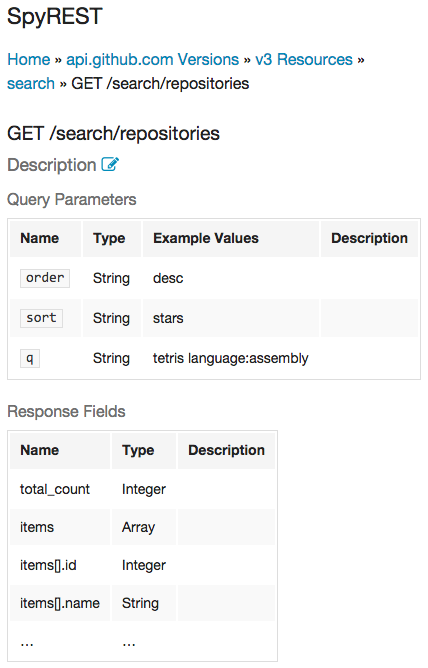
\includegraphics[width=\linewidth]{spyrest_header.png}
    \caption{API documentation summary section}
  \end{subfigure}
  \begin{subfigure}[t]{0.5\textwidth}
    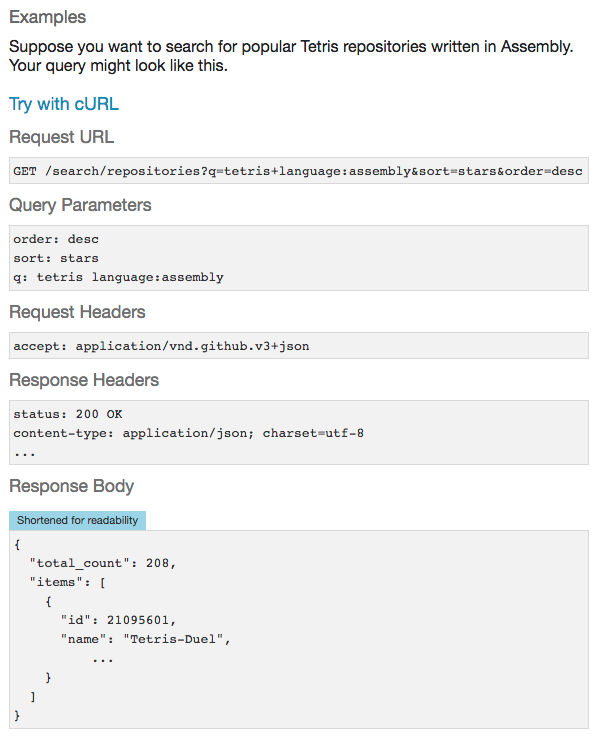
\includegraphics[width=\linewidth]{spyrest_examples.png}
    \caption{API documentation examples section}
  \end{subfigure}
  \caption{Screenshots of auto generated API documentation from SpyREST}
  \label{fig:spyrest_screenshots}
\end{figure*}

\textbf{The Web App:} The web app component further processes and presents auto generated documentation that is captured by Spy in the database. It also allows the users to edit or add custom content to the auto generated documentation. Additionally, the web app includes administration features such as user registration and SpyREST API key management. The features of the web app are discussed later in this paper in greater detail. The web app is written using the Ruby on Rails\footnote{http://rubyonrails.org/} framework primarily because of the first author's past experience using this framework.

The source code for both the Spy and Web app components are released as open source projects. Even though nodejs, MongoDB and Ruby on Rails are used for SpyREST implementation, the ideas that SpyREST realized are not dependent on these specific technologies.

\subsection{SpyREST Features} % (fold)

Now that we have explained the three SpyREST components and how they work, in the next paragraphs we discuss how SpyREST satisfies the aforementioned requirements.

\textbf{Automated RESTful API documentation:} The work flow for automated RESTful API documentation can be explained by the following steps: 1) API developer uses the Spy HTTP proxy to run example API calls, 2) The Spy records example API calls, 3) The Spy extracts meta information about the API call, 4) The Web app displays the auto generated documentation, 5) API developers can optionally customize the auto generated documentation.

Fig \ref{fig:spyrest_screenshots} shows screen shots  (content and presentation adapted for brevity) of fragments from of an auto generated documentation solely based on an example API call to URL \url{https://api.github.com/search/repositories?q=tetris+language:assembly&sort=stars&order=desc} with a custom header ``x-spy-rest-description'' to provide the short description for the example.

The auto-generated API documentation features a summary section. This section shows a breadcrumb containing the hierarchy of the API objects related to each API action to help users easily navigate the API documentation as a tree. This section also includes three tables that display the structure of query parameters, and request and response payloads. In addition to the structure, automated type detection is used to show the data type for each field in these tables. Example values are also automatically populated for query parameters.

The examples section on the API documentation shows all the recorded API examples for the given API action. For each example, it shows a short description, the request URL, request query parameters, and request and response headers and bodies. Because Spy filters out the ``authorization'' request header before saving the examples in the database, the documentation rendered by the web app excludes the secrets. As discussed before, the Spy also computes a ``strippedResponseBody'' by truncating large arrays in API responses to contain only two samples per array. The web app displays this ``strippedResponseBody'' to limit the verbosity on the auto-generated API documentation. Not shown in Fig. \ref{fig:spyrest_screenshots} for brevity, each example in the documentation also includes shows the SpyREST user that ran the API example and the time when it was generated.

\textbf{Example based:} As discussed earlier, SpyREST generated RESTful API documentation includes both the structure of the API objects and concrete examples for different use cases. The API examples are annotated with user provided descriptions through the custom headers that are otherwise hard to automatically infer. Because the Spy computes a hash digest for deduplication, replays of the same API example only updates the auto-generated documentation with the latest information allowing API developers to update the API documentation automatically when the API changes during development time. To record the examples in SpyREST, any REST API client can be used as long as it supports using a HTTP proxy to call the API.

\textbf{Executable documentation:} Because SpyREST keeps a copy of the API request information including URL, headers and request body, it can also recreate the example API calls that can be executed by users of the generated API documentation. Currently, it automatically generates executable test cases that can be run using cURL\footnote{http://curl.haxx.se/}. cURL is a command line based tool that can be used as a REST API client. The examples section on Fig. \ref{fig:spyrest_screenshots} shows a link titled ``Try with cURL'', on click of which the user gets a panel with am executable API call example reconstructed from the recorded data as shown in Fig. \ref{fig:curl}.

\begin{figure}[!tbh]
  \centering
  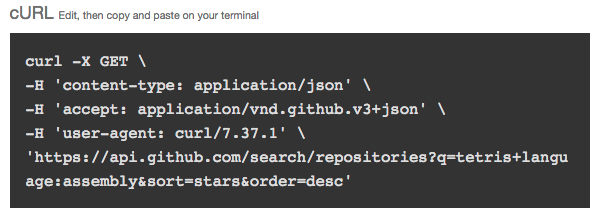
\includegraphics[width=\linewidth]{curl.png}
  \caption{Executable Examples in SpyREST using cURL}
  \label{fig:curl}
\end{figure}

This panel containing the executable API example is editable on the user interface. This allows the users to modify the API call if they need to customize the auto-generated API call. For example, to change the value of ``sort'' query parameter from ``desc'' to ``asc''  as shown in Fig. \ref{fig:curl}, a user can edit the text in this panel before executing the API example in cURL. Although not currently implemented, similar to cURL, SpyREST can generate executable tests targeting other REST API clients and programming languages since the required information to reconstruct an executable test is already available in the database.

\subsubsection{Version awareness}
  automatic version detection from headers, url, override

\subsubsection{Customizable}
  markdown editor

\textbf{Reusable:} Because SpyREST only relies on a HTTP proxy to auto-generate RESTful API documentation, it can be used to document RESTful APIs that are developed using any underlying technology. To feed SpyREST with data, any REST API client can be used as long as it supports connecting through a HTTP proxy server. This technology agnostic feature allows SpyREST to be a reusable RESTful API documentation tool.

SpyREST is offered as a SaaS tool that can be used to auto-generate and publish documentation of many different RESTful APIs.


\subsubsection{Collaborative}
  integrated commenting

\section{SpyREST In Action}

\section{Discussion}
How is it different from the existing tools?

Swagger
RESTdesc
RAML
API Blueprint


API call -- manual/bespoke implementation -- API Specification -- API documentation

API call -- automated record -- synthesize --  API documentation


\subsection{Limitations}
Pending user evaluation

% An example of a floating figure using the graphicx package.
% Note that \label must occur AFTER (or within) \caption.
% For figures, \caption should occur after the \includegraphics.
% Note that IEEEtran v1.7 and later has special internal code that
% is designed to preserve the operation of \label within \caption
% even when the captionsoff option is in effect. However, because
% of issues like this, it may be the safest practice to put all your
% \label just after \caption rather than within \caption{}.
%
% Reminder: the "draftcls" or "draftclsnofoot", not "draft", class
% option should be used if it is desired that the figures are to be
% displayed while in draft mode.
%
%\begin{figure}[!t]
%\centering
%\includegraphics[width=2.5in]{myfigure}
% where an .eps filename suffix will be assumed under latex,
% and a .pdf suffix will be assumed for pdflatex; or what has been declared
% via \DeclareGraphicsExtensions.
%\caption{Simulation Results}
%\label{fig_sim}
%\end{figure}

% Note that IEEE typically puts floats only at the top, even when this
% results in a large percentage of a column being occupied by floats.


% An example of a double column floating figure using two subfigures.
% (The subfig.sty package must be loaded for this to work.)
% The subfigure \label commands are set within each subfloat command, the
% \label for the overall figure must come after \caption.
% \hfil must be used as a separator to get equal spacing.
% The subfigure.sty package works much the same way, except \subfigure is
% used instead of \subfloat.
%
%\begin{figure*}[!t]
%\centerline{\subfloat[Case I]\includegraphics[width=2.5in]{subfigcase1}%
%\label{fig_first_case}}
%\hfil
%\subfloat[Case II]{\includegraphics[width=2.5in]{subfigcase2}%
%\label{fig_second_case}}}
%\caption{Simulation results}
%\label{fig_sim}
%\end{figure*}
%
% Note that often IEEE papers with subfigures do not employ subfigure
% captions (using the optional argument to \subfloat), but instead will
% reference/describe all of them (a), (b), etc., within the main caption.


% An example of a floating table. Note that, for IEEE style tables, the
% \caption command should come BEFORE the table. Table text will default to
% \footnotesize as IEEE normally uses this smaller font for tables.
% The \label must come after \caption as always.
%
%\begin{table}[!t]
%% increase table row spacing, adjust to taste
%\renewcommand{\arraystretch}{1.3}
% if using array.sty, it might be a good idea to tweak the value of
% \extrarowheight as needed to properly center the text within the cells
%\caption{An Example of a Table}
%\label{table_example}
%\centering
%% Some packages, such as MDW tools, offer better commands for making tables
%% than the plain LaTeX2e tabular which is used here.
%\begin{tabular}{|c||c|}
%\hline
%One & Two\\
%\hline
%Three & Four\\
%\hline
%\end{tabular}
%\end{table}


% Note that IEEE does not put floats in the very first column - or typically
% anywhere on the first page for that matter. Also, in-text middle ("here")
% positioning is not used. Most IEEE journals/conferences use top floats
% exclusively. Note that, LaTeX2e, unlike IEEE journals/conferences, places
% footnotes above bottom floats. This can be corrected via the \fnbelowfloat
% command of the stfloats package.



\section{Conclusion}
The conclusion goes here.




% conference papers do not normally have an appendix


% use section* for acknowledgement
\section*{Acknowledgment}


The authors would like to thank...





% trigger a \newpage just before the given reference
% number - used to balance the columns on the last page
% adjust value as needed - may need to be readjusted if
% the document is modified later
%\IEEEtriggeratref{8}
% The "triggered" command can be changed if desired:
%\IEEEtriggercmd{\enlargethispage{-5in}}

% references section

% can use a bibliography generated by BibTeX as a .bbl file
% BibTeX documentation can be easily obtained at:
% http://www.ctan.org/tex-archive/biblio/bibtex/contrib/doc/
% The IEEEtran BibTeX style support page is at:
% http://www.michaelshell.org/tex/ieeetran/bibtex/
%\bibliographystyle{IEEEtran}
% argument is your BibTeX string definitions and bibliography database(s)
%\bibliography{IEEEabrv,../bib/paper}
%
% <OR> manually copy in the resultant .bbl file
% set second argument of \begin to the number of references
% (used to reserve space for the reference number labels box)
\begin{thebibliography}{1}

\bibitem{IEEEhowto:kopka}
H.~Kopka and P.~W. Daly, \emph{A Guide to \LaTeX}, 3rd~ed.\hskip 1em plus
  0.5em minus 0.4em\relax Harlow, England: Addison-Wesley, 1999.

\end{thebibliography}




% that's all folks
\end{document}


